\documentclass{article}
\usepackage[utf8]{inputenc}
\usepackage{subfig}
\usepackage{amsmath}

\usepackage{graphicx}
\usepackage[a3paper, landscape, margin=0.5cm]{geometry}

\thispagestyle{empty}
% \renewcommand{\thesubfigure}{\roman{subfigure}}
\begin{document}

\begin{figure}[t]
        \centering
        \subfloat[vertical caustics]{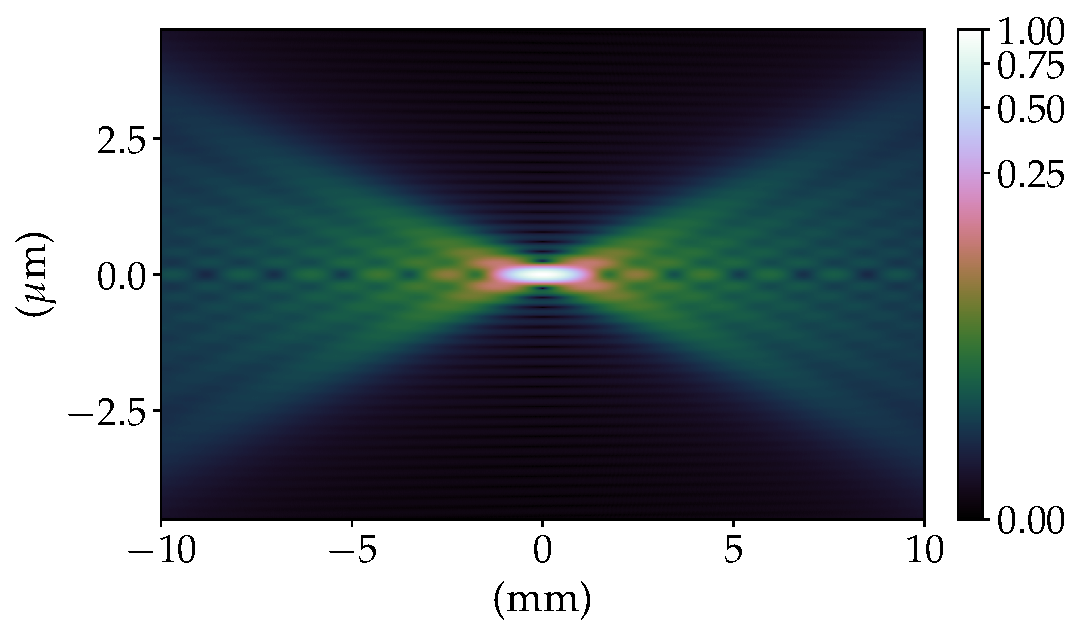
\includegraphics[height=3.4cm]{figures/ch05/CDn_vs_CDnStack/Be_ideal_8p0keV_d0p0mm_n10_intensity_cstc_Y_cstc_2D.pdf}}\hspace{0.1cm}
        \subfloat[PSF phase (rad)]{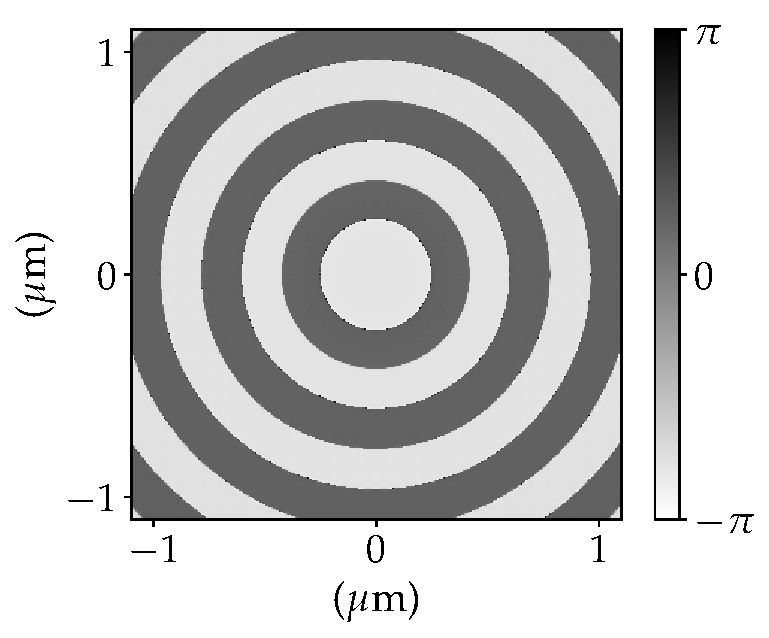
\includegraphics[height=3.5cm]{figures/ch05/CDn_vs_CDnStack/Be_ideal_8p0keV_d0p0mm_n10_phase_phase_2D.pdf}}\hspace{0.1cm}
        \subfloat[PSF intensity]{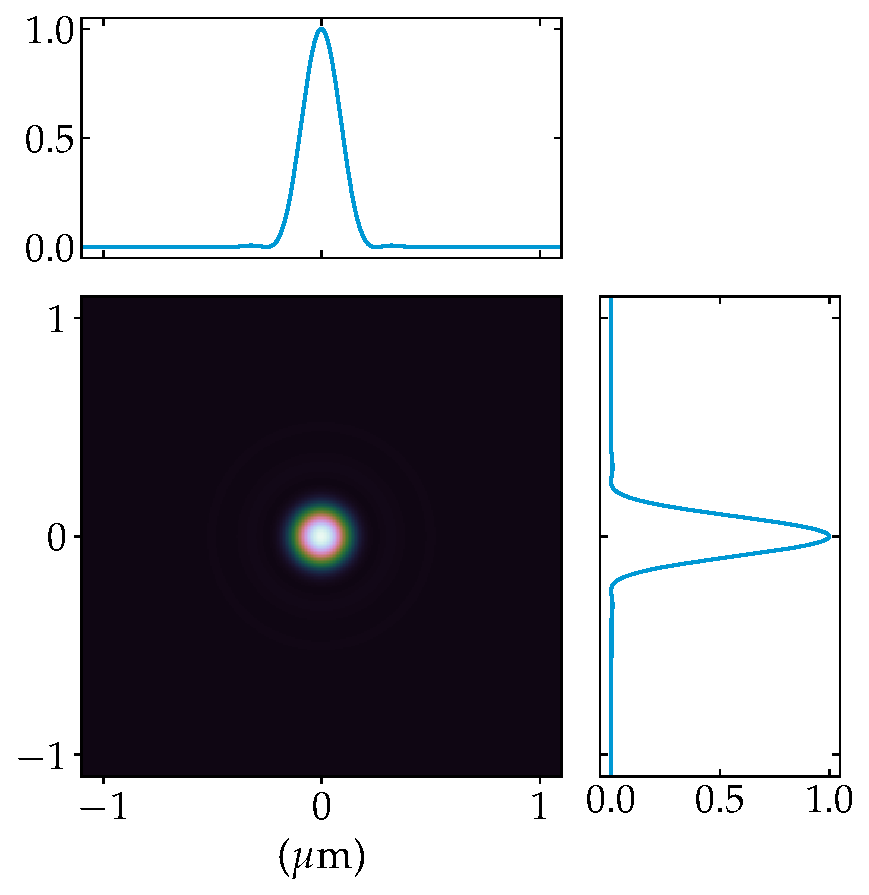
\includegraphics[height=5cm]{figures/ch05/CDn_vs_CDnStack/Be_ideal_8p0keV_d0p0mm_n10_intensity_intensity_2D.pdf}}\hspace{0.1cm}
        \subfloat[source image]{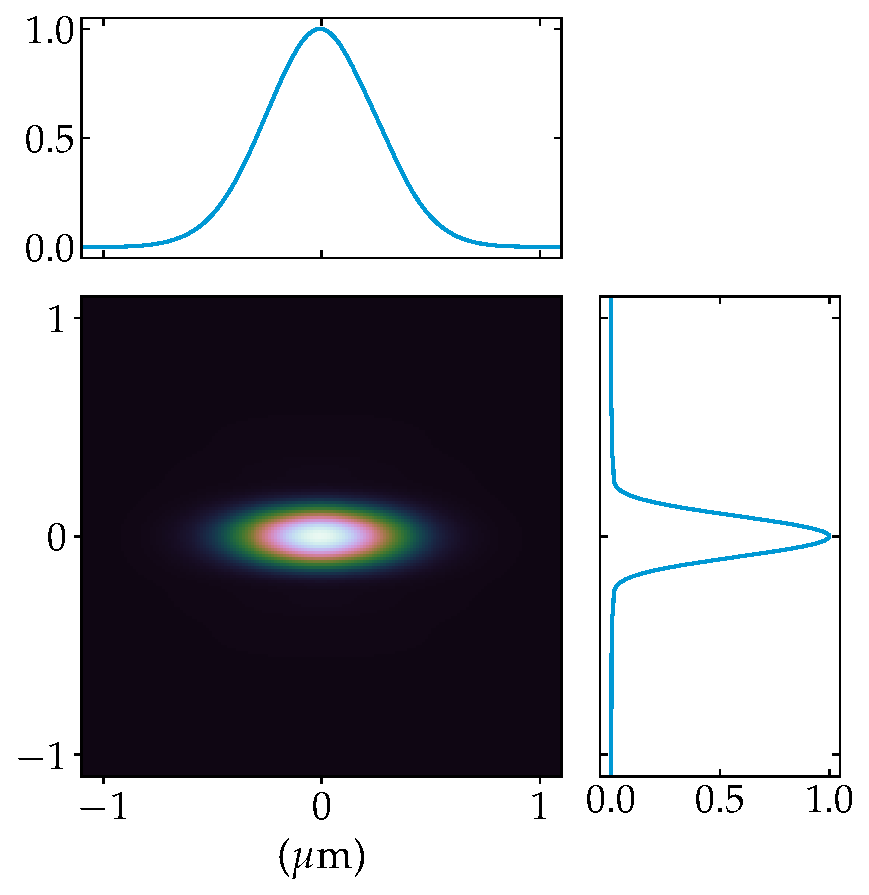
\includegraphics[height=5cm]{figures/ch05/CDn_vs_CDnStack/Be_ideal_8keV_d0p0mm_10k_ME_intensity_intensity_2D.pdf}}
        \caption*{ideal stacked lenses}\vspace{0.3cm}\setcounter{subfigure}{0}
        \subfloat[vertical caustics]{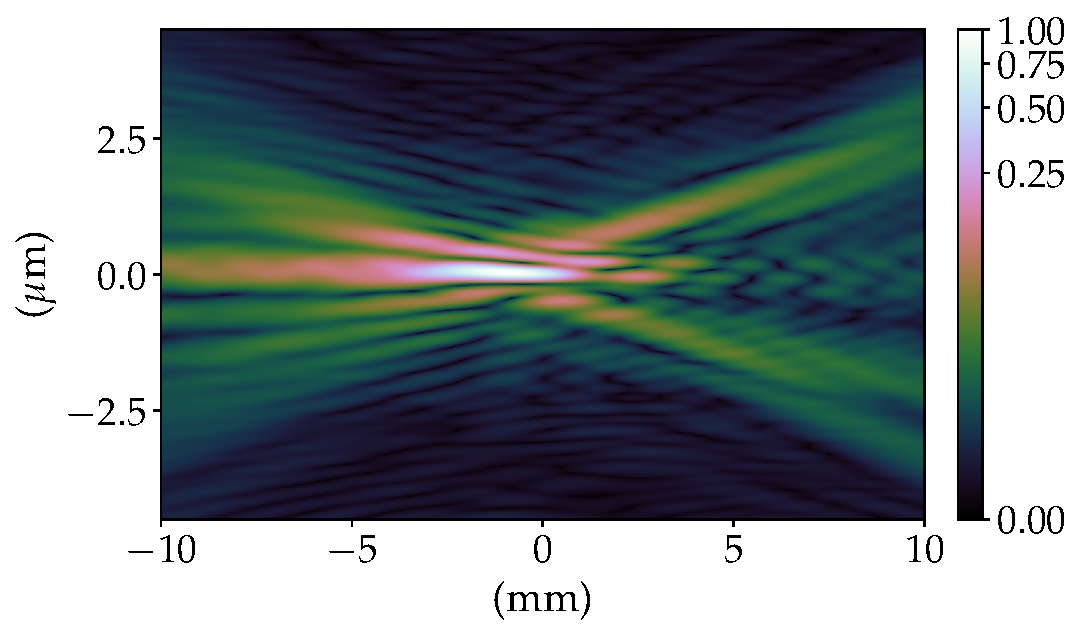
\includegraphics[height=3.4cm]{figures/ch05/CDn_vs_CDnStack/Be_CDo_8p0keV_d0p0mm_n10_intensity_cstc_Y_cstc_2D.pdf}}\hspace{0.1cm}
        \subfloat[PSF phase (rad)]{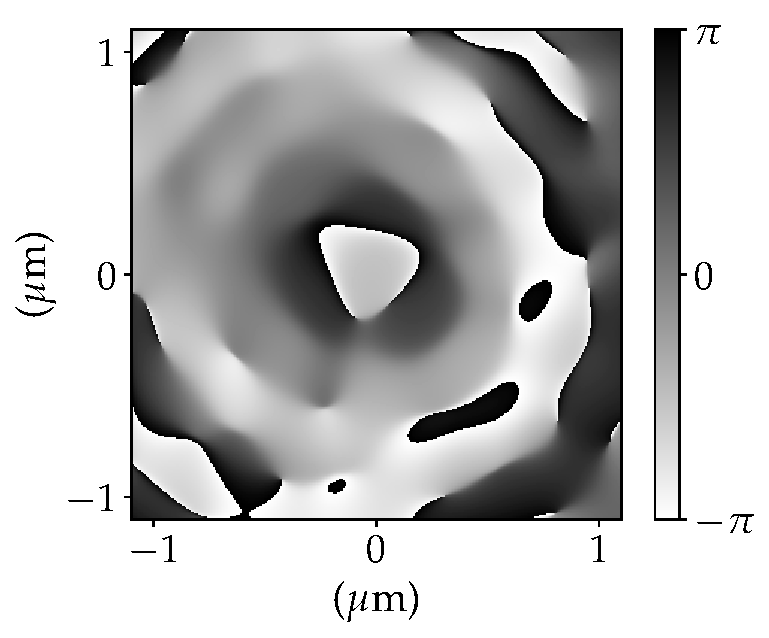
\includegraphics[height=3.5cm]{figures/ch05/CDn_vs_CDnStack/Be_CDo_8p0keV_d0p0mm_n10_phase_phase_2D.pdf}}\hspace{0.1cm}
        \subfloat[PSF intensity]{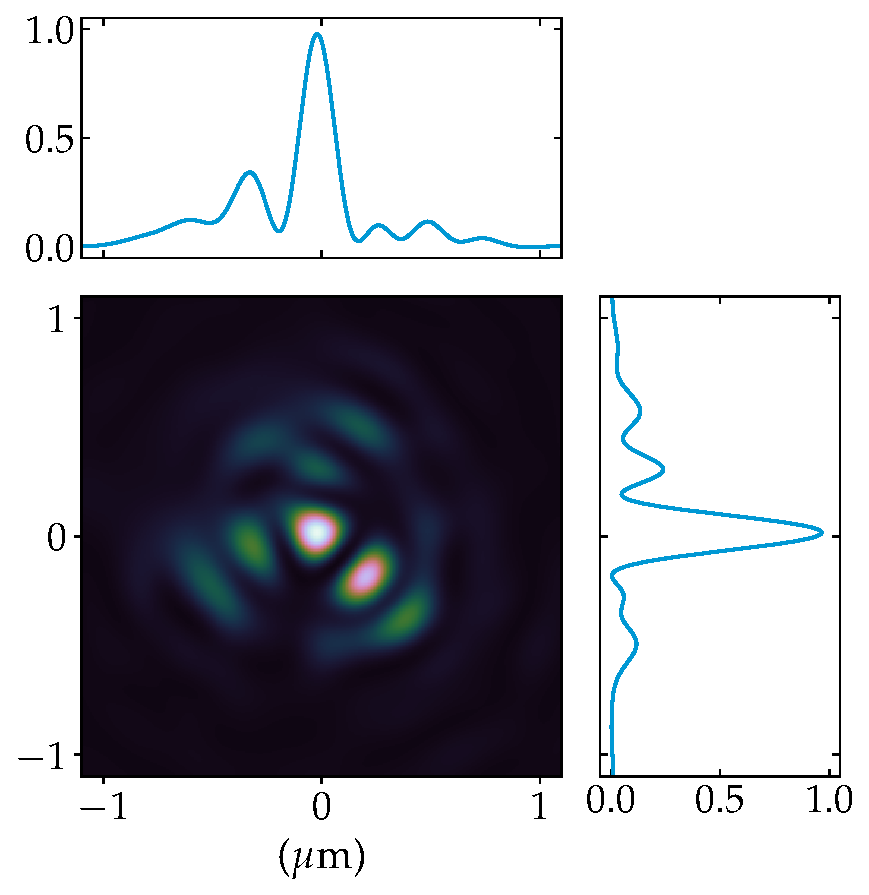
\includegraphics[height=5cm]{figures/ch05/CDn_vs_CDnStack/Be_CDo_8p0keV_d0p0mm_n10_intensity_intensity_2D.pdf}}\hspace{0.1cm}
        \subfloat[source image]{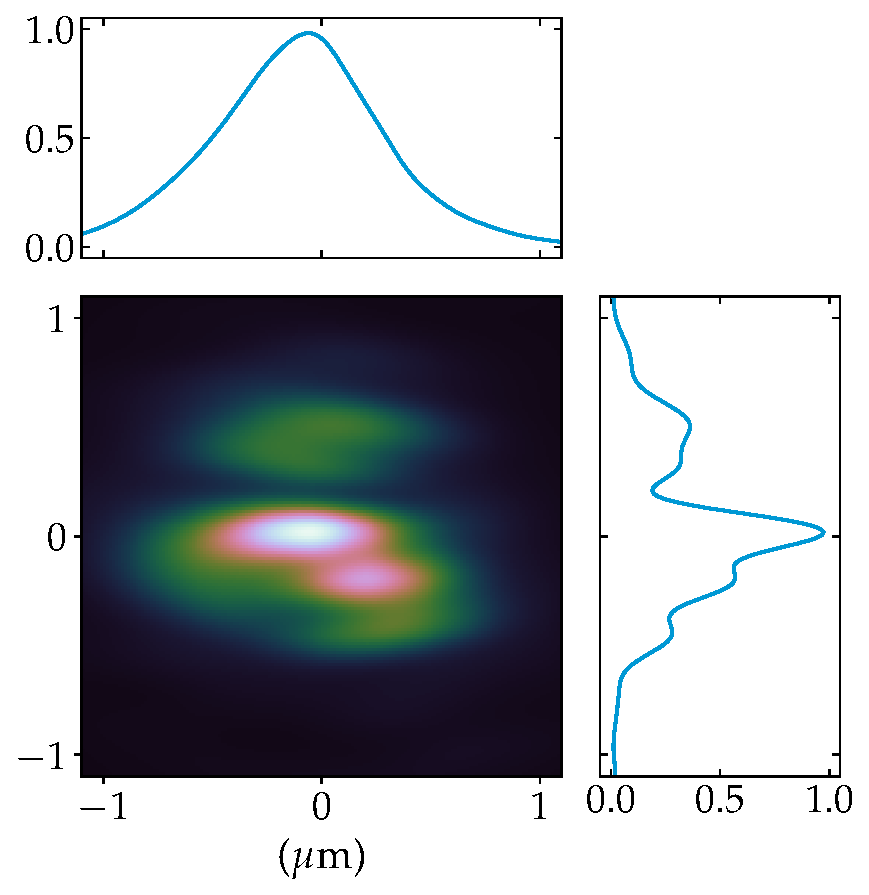
\includegraphics[height=5cm]{figures/ch05/CDn_vs_CDnStack/Be_CDo_8keV_d0p0mm_10k_ME_intensity_intensity_2D.pdf}}
        \caption*{artificially stacked lenses L11-L20}\vspace{0.3cm}\setcounter{subfigure}{0}
        \subfloat[vertical caustics]{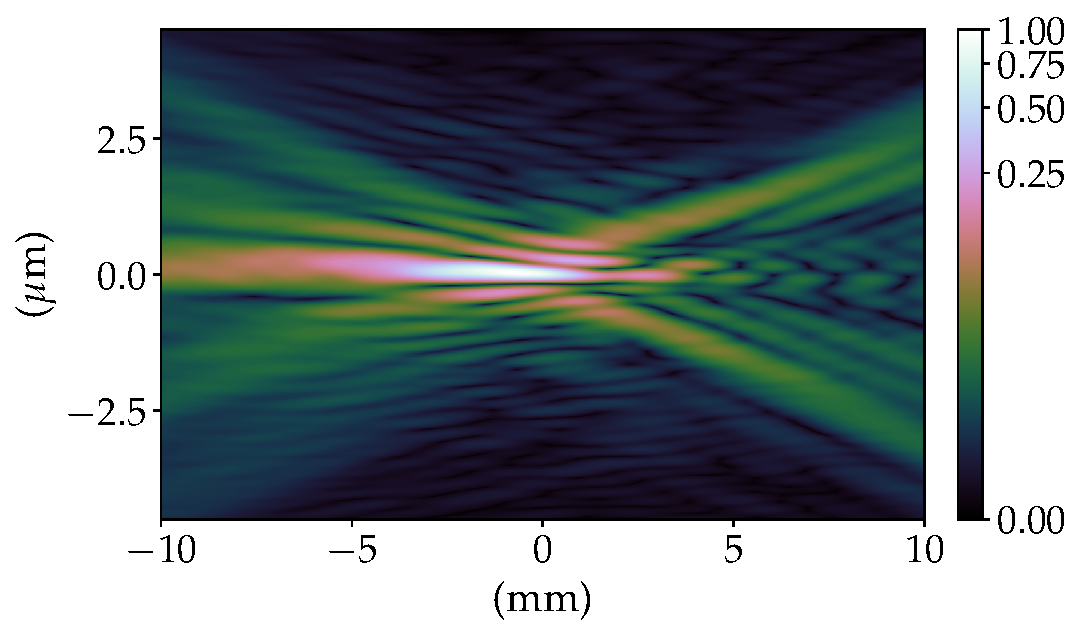
\includegraphics[height=3.4cm]{figures/ch05/CDn_vs_CDnStack/Be_CDo_stack_8p0keV_d0p0mm_n10_intensity_cstc_Y_cstc_2D.pdf}}\hspace{0.1cm}
        \subfloat[PSF phase (rad)]{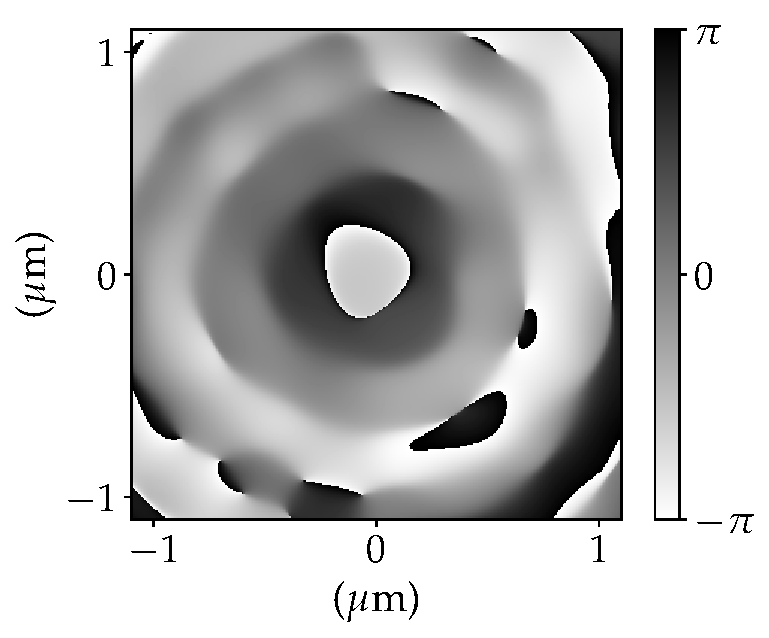
\includegraphics[height=3.5cm]{figures/ch05/CDn_vs_CDnStack/Be_CDo_stack_8p0keV_d0p0mm_n10_phase_phase_2D.pdf}}\hspace{0.1cm}
        \subfloat[PSF intensity]{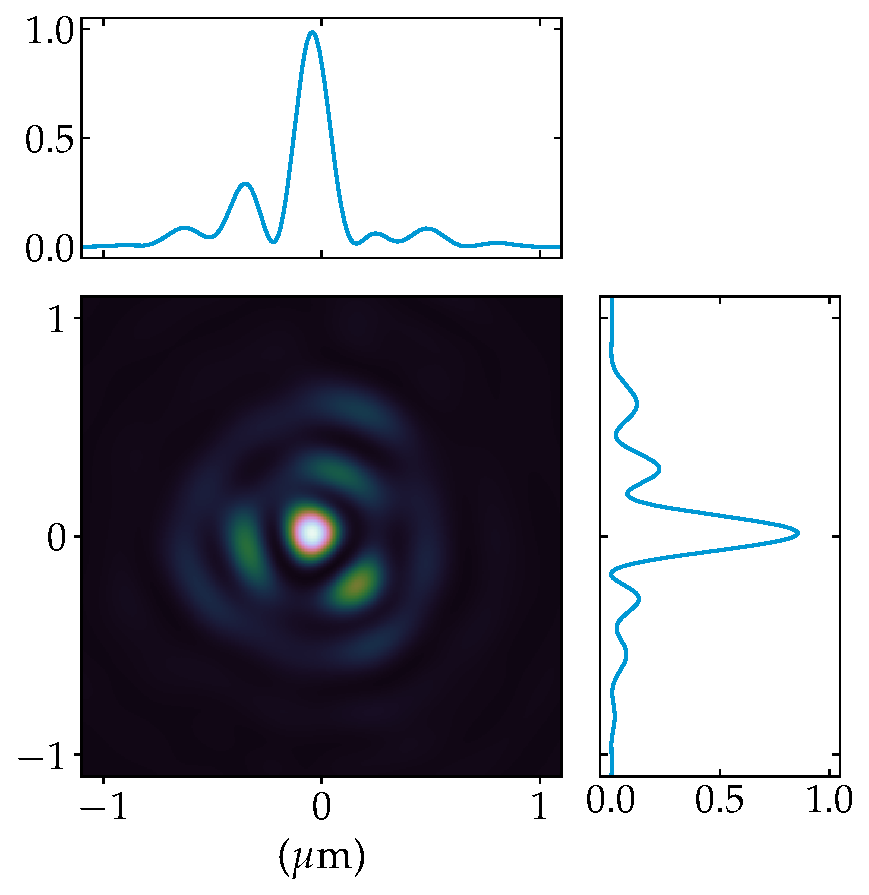
\includegraphics[height=5cm]{figures/ch05/CDn_vs_CDnStack/Be_CDo_stack_8p0keV_d0p0mm_n10_intensity_intensity_2D.pdf}}\hspace{0.1cm}
        \subfloat[source image]{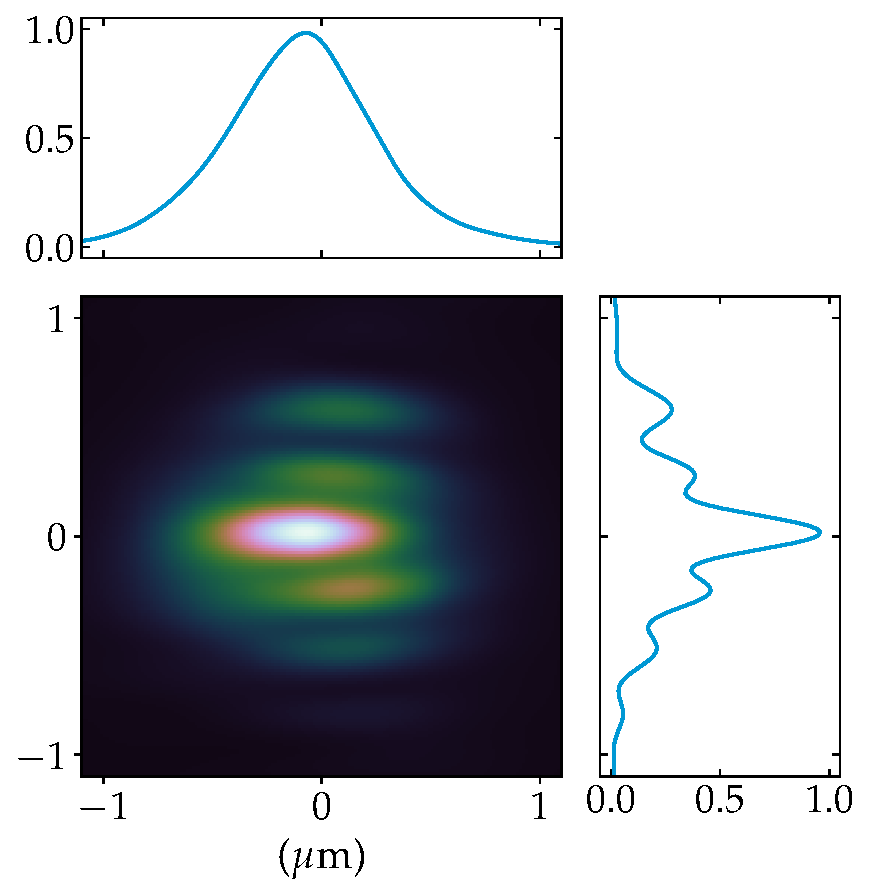
\includegraphics[height=5cm]{figures/ch05/CDn_vs_CDnStack/Be_CDo_Stack_8keV_d0p0mm_10k_ME_intensity_intensity_2D.pdf}}
        \caption*{stack 2}\vspace{0.3cm}
        \subfloat[fully-coherent]{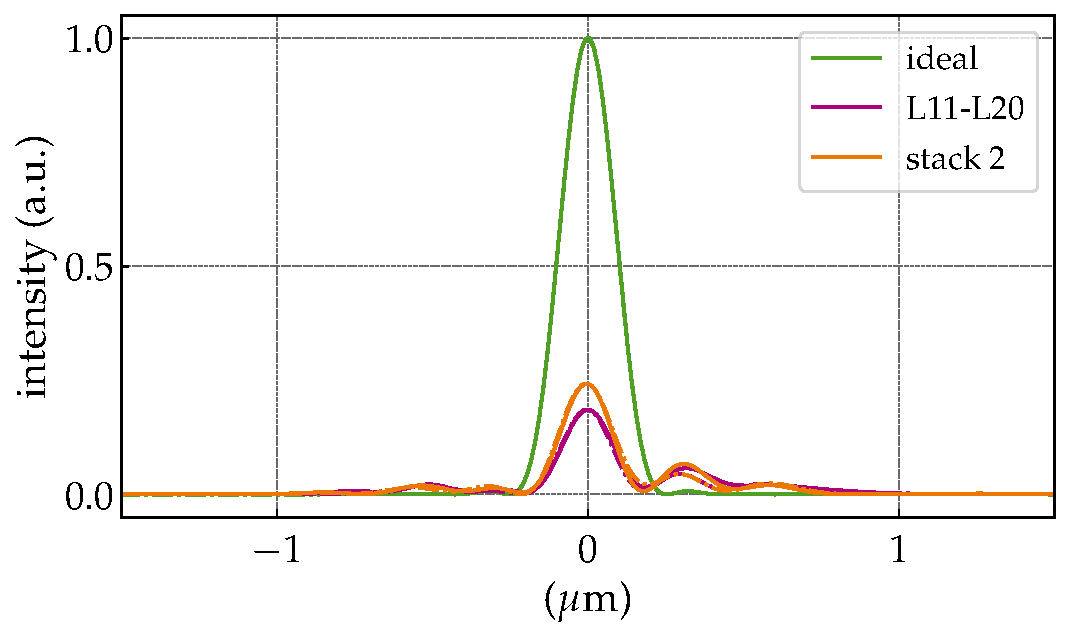
\includegraphics[height=3.3cm]{figures/ch05/CDn_vs_CDnStack/Strehl_SE_CDo_vs_CDnStack.pdf}}\hspace{0.1cm}
        \subfloat[partially-coherent]{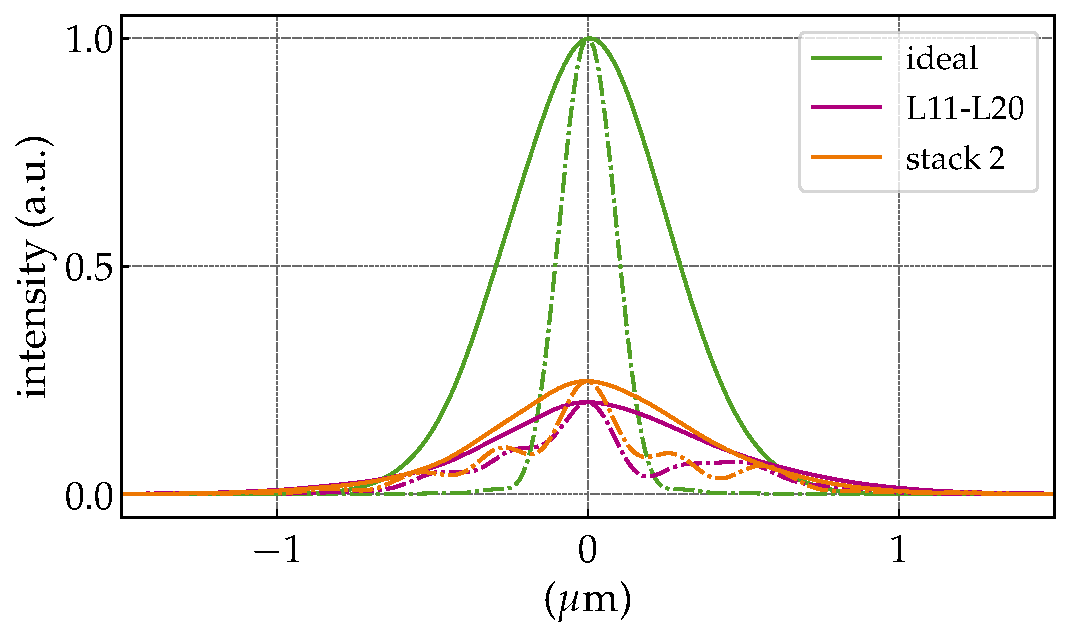
\includegraphics[height=3.3cm]{figures/ch05/CDn_vs_CDnStack/Strehl_ME_CDo_vs_CDnStack.pdf}}
       \caption*{Strehl ratio}
\end{figure}
\end{document}